\scanpage{183}
Soit $\mathcal M$ une catégorie de motifs géométriques, \inserted{\figure{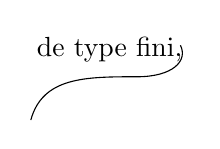
\begin{tikzpicture}[x=1cm,y=1cm]\node at (0,.3) {de type fini,};\draw (-1,-.6) .. controls (-.85,-.05) and (-.3,-.05) .. (.35,-.05) .. controls (.8,-.05) and (1,.15) .. (.9,.35);\end{tikzpicture}}} sur le préschéma $S$ de type fini sur $\mathbf Z$. Pour simplifier, supposons que les degrés de $\mathcal M$ soient pairs (sinon, il sera possible, pour \deleted{la plupart des} \inserted{certaines} questions de distribution des Frobenius, de remplacer $\mathcal M$ par $\mathcal M^{\mathrm{pair}}$). Tout choix d'un pt fermé $s\in S$ permet donc, de définir des (une collection de) ``$\mathbf R$-points Motiviques'' \deleted{\unsure{point de vue}''} \inserted{de $\mathcal M$}.

Pour fixer les idées, choisissons un pt $\mathbf R$-motivique de $\mathcal M$, d'où un gpe physique $G_{\mathbf R}$ sur $\mathbf R$.

Il y a lieu de \deleted{dupliquer} \inserted{démultiplier} les point \inserted{\figure{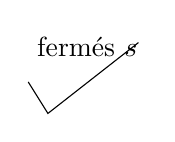
\begin{tikzpicture}[x=1cm,y=1cm]\node at (0,.3) {fermés $s$};\draw (-.75,-.15)--(-.5,-.55)--(.65,.35);\end{tikzpicture}}} de $S$, en formant les couples $s'=(s,\unsure{i|i'})$, où $s\in S^0$, et
\margin{l'exposant $0$ désigne des pts \uline{fermés}}
$i_{\deleted{\unsure{s|x}}}\colon G_{m\,\mathbf C}-G(s)_{\mathbf C}$ est de type \deleted{\unsure{divisé|désigné}} préférentiel --- $G(s)$ désigne le gpe de Galois motivique associé à $\mathcal M_s$.

\deleted{Alors} Soit $S'$ l'ens de ces couples. A tout $s'\in S'$ est associé un $\mathbf R$-point motivique de $\mathcal M$, \deleted{d'où un} déterminé à isom près, d'où un $\zeta(s')\in H^1(\mathbf R,\deleted{F}G_{\mathbf R}^{\mathrm{or}})$, où $G^{\mathrm{or}}$ est le noyau de $G_{\mathbf R}^0\xrightarrow{\varepsilon}G_m$. De plus, si $G_{\mathbf R}^{\zeta(s')}$ est ``le'' gpe déduit de $G_{\mathbf R}$ par torsion par $\zeta(s')$, on obtient un hom
\[
u(s')\colon G(s')_{\deleted{\unsure{R|k}}\mathbf R}=G(s)_{\mathbf R}\longrightarrow G_{\mathbf R}^{\zeta(s')}
\]
compatible avec $\varepsilon_{\mathbf R},J_{\mathbf R}$, et déterminé en fait mod \deleted{\unsure{automorphisme|automorphismes}} \inserted{conjugaison} \deleted{\unsure{intérieur|intérieurs}} par un élément de $G_{\mathbf R}^{\mathrm{or}}(\mathbf R)$.
\margin{182}
